\scanpage{374}
\uuline{Foncteurs derives droits de Sym.}
\[
H^*(X,R)\simeq\underbrace{H^*(X,\mathbb F_p)}\otimes_{\mathbb F_p}R
\]
$\Theta\in\mathscr A=$ \unsure{algebre|algèbre} de Steenrod
\[
\begin{aligned}
\underbrace{P_R^i}_{\substack{\text{construit}\\\text{par Steenrod}}}
 &=P^i\otimes1\qquad i>0\qquad 2i(p-1)\\
\text{\textcircled{$P_R^0$}}&=\underbrace{P^0}_{1}\otimes F
\end{aligned}
\]
\[
G_a\otimes(\Lambda^n\Psi)\qquad G_a=\text{Fais structural de }(\mathrm{Sch}/\mathbb F_p)
\]
\figure{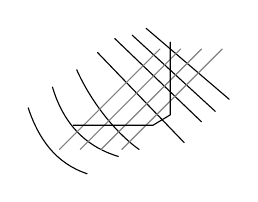
\begin{tikzpicture}[scale=.44,line cap=round]
\draw (0,.2)..controls (.3,-.7) and (.8,-1.4)..(1.7,-1.7);
\draw (.7,.8)..controls (1,-.2) and (1.6,-.9)..(2.6,-1.2);
\draw (1.4,1.3)..controls (1.8,.4) and (2.5,-.5)..(3.2,-1);
\draw (2,1.8)--(4.5,-.8); \draw (2.5,2.2)--(5,-.2);
\draw (3,2.3)--(5.4,.1); \draw (3.4,2.5)--(5.8,.45);
\foreach \x in {0,.6,1.2,1.8}{\draw[gray,thin] (\x+.9,-1)--(\x+3.8,1.9);}
\draw (1.3,-.3)--(3.6,-.3)--(4.1,0)--(4.1,2.1);
\end{tikzpicture}}
\[
\begin{aligned}
H^*(K(G_a,n),G_a)&=\text{\unsure{Cl.|\ensuremath{\mathscr A\cdot}} les op}\\
H^*(\mathbb Z[K(G_a,n)],G_a)&
\end{aligned}
\]
% slanted
Illusie $\unsure{X\in\text{cat }D,(T)|X\text{ cat }D,(T)|X\in\mathrm{ob}\,D_{\bullet}(T)}$ cat derivée des fais simpl\qquad $F$ objet abelien
\diagram{\begin{tikzcd}[ampersand replacement=\&,column sep=small]
\&H^*(X,F^{\unsure{*|\prime}})=[X,K(F,n)]\\
H^j(X_i,F)\arrow[ur,Rightarrow]\& X'\arrow[r]\arrow[d] \& K(F,n)\\
\&X
\end{tikzcd}}
\margin{Epstein L. Operations in homological algebra\par Invent. Math. 1 (1966)}

Illusie p 69\qquad 3.2.1.19 -- 3.2.1.18
\[
\begin{aligned}
&\operatorname{Ext}^{p}(N(X),F)=\lim_{\substack{X'\to X\\\mathrm{qis}\\\text{fibrant}}}[X',K(F,p)]\\
&\text{dit }''\, H^p(X,F)
\end{aligned}
\]
\[
\operatorname{Ext}^p(N(-),F)\longrightarrow\operatorname{Ext}^q(N(\ ),G)
\]
% slanted
Op coh de type $(F,p,G,q)$ sont class par $H^q(K(F,p),G)$
\margin{$\unsure{Z|z|\mathbb Z}X\xrightarrow{f}K(A,q$}

\[
H^n(K(G_a,m),G_a)=R^n\operatorname{Sym}(\mathbb F_p[m])
=\text{dual de }L^n\Gamma\,\deleted{\unsure{\mathrm{Hom}|\mathrm{Sym}}}(\mathbb F_p[m])
\]
\uline{Theoreme} : Soit $\mathscr A$ l'algebre sur $\mathbb F_p$ eng par $P^i$\qquad
$\deg P^i=2i(p-1)$\qquad $i\geq0$ sat aux relations d'Adem (mais non à $P^0=1$).
\[
H^*(K(\deleted{G_a}\mathcal O,m),\deleted{G_a}\mathcal O)
\]
est l'alg anticomm libre engendrée par les monomes admissibles de $\mathscr A$ d'exces $<n$.
\margin{$H^*(K(\mathbb F_{p^h},n),\mathbb F_{p^h})$}

\uline{Dém} : Comme dans le cas classique, il suffit de calculer $H^*(K(G_a,1),G_a)$ et de grimper en utilisant le th de Borel et la suite sp de Leray associée à
\diagram{\begin{tikzcd}[ampersand replacement=\&]
K(G_a,n-1)\arrow[r]\& *\arrow[d]\\
\&K(G_a,n)
\end{tikzcd}}
$\downarrow$\quad Lazard : Coh de l'analyseur classique dans ``Lois de groupes formels et analyseurs'' Ann ENS

\margin{$R$ anneau de car $p\unsure{>|{\geq}}0$\par $H^*(K(R,n),R)=$ Alg anticomm libre /$R$ eng par $\operatorname{Hom}_{\rm Ab}(R,R)$-module libre eng par les monomes admissibles $f\in\operatorname{Hom}(R,R)$}
\margin{$\oplus\ P^If\iota_n$\par $\underset{\rotatebox{90}{$\in$}\,x}{H^*(X,\mathcal O)}\longrightarrow\underset{P^Ix}{H^*(X,\mathcal O)}$\par $\mathrm{Hom}$}
\diagram{\begin{tikzcd}[ampersand replacement=\&,row sep=small]
G_a^3\&G_a\times G_a\&G_a\\
\&\&\deleted{\operatorname{Sym}\mathbb F_p}\\
k[x,y,z]\&k[x,y]\arrow[l]\&k[x]\arrow[l]
\end{tikzcd}}
\[
\begin{aligned}
\iota_1&\in H^1(K(G_a,1),G_a)\\
\text{Witt}\ \longleftarrow\ \beta&\in H^2(K(G_a,1),G_a)\\
0\to G_a\to W_2&\to G_a\to0\\
0\to\mathbb Z/p\to\mathbb Z/p^2&\to\mathbb Z/p\to0
\end{aligned}
\]
On se ramène au calcul de
\diagram{\begin{tikzcd}[ampersand replacement=\&]
\&H^*(K(\mathbb F_{p^h};1),\mathbb F_{p^h})\\
x\in H^n(K(\mathcal O,m),\mathcal O)\arrow[ur]\& {}\\
K(\mathcal O,m)\arrow[r]\&K(\mathcal O,n)\\
K(R,m)\arrow[r]\&K(R,n)\qquad\forall R/\mathbb F_p
\end{tikzcd}}
\noindent\rule{.8\linewidth}{.3pt}

représenté par des polynomes de deg $<p^h$ en chaque var
\[
x\in H^*(K(\mathcal O,n),\mathcal O)_h\xrightarrow{\text{injective}}H^*(K(\mathbb F_{p^h},n),\mathbb F_{p^h})
\]
% archive sheet number: 376
